%!TEX root = ../../Heun_Dale_Haney_A_dynamic_approach_to_input_output_modeling.tex
%%%%%%%%%%%%%%%%%%%%% chapter.tex %%%%%%%%%%%%%%%%%%%%%%%%%%%%%%%%%
%
% sample chapter
%
% Use this file as a template for your own input.
%
%%%%%%%%%%%%%%%%%%%%%%%% Springer-Verlag %%%%%%%%%%%%%%%%%%%%%%%%%%
%\motto{Use the template \emph{chapter.tex} to style the various elements of your chapter content.}
\chapter{Introduction}
% use \chaptermark{}
% to alter or adjust the chapter heading in the running head
\chaptermark{Introduction}
% Always give a unique label
\label{chap:intro}

\abstract*{[NEED TO ADD ABSTRACT HERE]}

%% \abstract{Each chapter should be preceded by an abstract (10--15 lines long) that summarizes the content. The abstract will appear \textit{online} at \url{www.SpringerLink.com} and be available with unrestricted access. This allows unregistered users to read the abstract as a teaser for the complete chapter. As a general rule the abstracts will not appear in the printed version of your book unless it is the style of your particular book or that of the series to which your book belongs.\newline\indent
%% Please use the 'starred' version of the new Springer \texttt{abstract} command for typesetting the text of the online abstracts (cf. source file of this chapter template \texttt{abstract}) and include them with the source files of your manuscript. Use the plain \texttt{abstract} command if the abstract is also to appear in the printed version of the book.}

%% Use the template \emph{chapter.tex} together with the Springer document class SVMono (monograph-type books) or SVMult (edited books) to style the various elements of your chapter content in the Springer layout.

DISCUSSION POINTS
\begin{itemize}
\item{Important to highlight difference between material and financial depreciation.}
\item{Embodied energy flows with material, not with dollars}
\item{Financial depreciation is typically (under normal circumstances) a leading indicator of material depreciation}
\item{Prior to accumulation, embodied energy is passed into products.}
\item{Is `society' the best word – `final consumption?'}
\item{Do we use energy circuit language?}
\item{For economists, capital is only in the productive sector, $\dot{K}_{i2}$ flows would be `consumer durables'}
\item{Housing is `residential capital'}
\end{itemize}

\section{Traditional view of economy}

The traditional economic flows accounts for gross payments 
from the household sector for goods and services that flow 
from the production sector and payments 
from the production sector for wages and rents to the household sector.

\section{Brief history of input-output (I-O) modeling}

Input-output analysis, developed by Wassilly Leontief in the 1930s 
as an extension to the work of Quesnay and Walras \cite{Leontief1936}, 
is of primary importance in national accounting, 
allowing determination of the structure of an economy as well as, 
among other things, 
calculation of a nation's gross domestic product (GDP), 
the predominant measure of economic activity.

\section{Basic I-O method}

The basic premise of the I-O method, as depicted in Figure \ref{fig:basic_unit}A, is that each economic sector takes in factors of production from other sectors (and possibly itself) to produce an economic good at some rate. For example, the automotive sector takes in steel, rubber, glass, etc. and produces a number of cars per year. In contrast to high-level economic growth models that include only a few factors of production (such as land, capital, and labor), the I-O analysis technique allows many differentiated factors of production and raw material feedstocks. \cite{Costanza:1980ww} In I-O frameworks, each factor of production is considered to be the output from a sector of the economy. As will be discussed later [MAKE SURE TO DISCUSS THIS LATER!], the traditional primary factors of production (land, capital, and labor) are not \emph{flows} into the production processes. Rather, they are \emph{stocks} that, when present, allow factors of production (steel, rubber, and glass) to be transformed into final products (automobiles). The quantity and quality of these stocks determine the quantity and quality of their flow of productive services.


In addition to the productive services provided by stocks of land, capital, and labor,
a flow of energy\footnote{Or, more precisely, the degradation of an exergetic gradient/destruction of exergy.} is  required for economic activity. These energy flows originate from the natural environment, recognition of which has provoked researchers from fields of net energy analysis (NEA), material flow analysis (MFA), industrial ecology (IE) and life-cycle assessment (LCA) to extend the traditional (Leontief) input-output framework to include important material and energy flows to and from the environment, as depicted in Figure \ref{fig:basic_unit_B} \cite{Carter1974,Bullard1975,Bullard1976a,Herendeen1978,Costanza:1980ww,Casler1984,Joshi1999,Suh2009}. While the Leontief I-O approach relies exclusively on monetary units to represent value flows among sectors of an economy, the key insight of these extensions of the Leontief I-O framework is to rely upon physical units (especially energy units of joules) to represent some of the value flows among economic sectors. In doing so, energy and material intensities of value flows can be estimated. This extended approach is depicted in Figure \ref{fig:basic_unit}B. 

Both the original Leontief I-O framework and the extensions cited above assume steady-state conditions in an economy, i.e., flows of value and material into and out of each economic sector are in balance. Dynamic or transient behavior of the economic system is not considered. Thus, there is no accumulation of economic factors or embodied energy within any of the sectors. The analysis techniques provide ``snapshots'' of economic activity at an instant in time.

[MIK'S NEW ADDITION]

Assuming no accumulation of materials, within economic sectors or society itself, is tantamount to assuming that \emph{all} material flows through the economy are directed toward the production of non-durable goods. However, evidence of the durability of goods and the accumulation of materials surrounds us. Furthermore, energy was required to both fabricate and emplace the durable goods and infrastructure of modern economies. (The energy it took to create the durable goods and infrastructure can be considered ``embodied'' within the built environment, a point to which we will return in detail later). As Georgescu-Roegen notes, ``in the everyday world one cannot possibly cross a river only on the flow of maintenance materials of a non-existent bridge.'' \cite{G-R1975}. 

Analysis methods that neglect the accumulation of materials and embodied energy in the durable goods and infrastructure of the everyday world lack explanatory power. Such models can tell us how at what rates materials and energy are required to \emph{use} our built environment. But, such models cannot tell us \emph{how} the built environment came to be (and how much energy was required to construct it) or \emph{why} flows of goods are needed. To use Georgescu-Roegen's imagery, models that neglect accumulation fail to explain why we need any material flows to maintain a non-existent bridge. Stocks of accumulated materials (capital, appliances, even people) are the drivers of demand. It is to service their needs and wants that we put the economy to work. %[THESE LAST TWO SENTENCES ARE EXCELLENT! --MKH] 

Because economic activity requires energy, we need to understand the way energy flows through economies. The steady-state I-O techniques of Bullard, Herendeen, and others\cite{Bullard1975,Herendeen1978} [REFERENCES NEEDED --MKH] offer a means to that end. We contend, however, that these techniques need to be extended and modified to include transient effects that arise when durability of goods and infrastructure (and associated embodied energy) are considered. This paper attempts to address that need.

\begin{figure}[!ht]
\centering{}
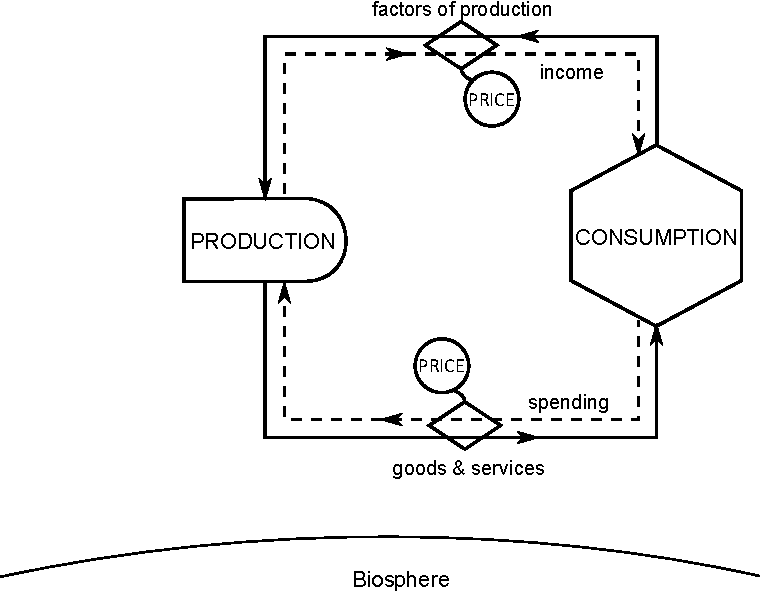
\includegraphics[width=\linewidth]{Part_0/Chapter_Introduction/images/Perpetual_motion_1.pdf}
\caption[The traditional economic model of the economy]{The traditional model represents the economy as a circular flow of goods and services between two sectors. The producers manufacture goods and services by taking in labor and capital. The consumers exchange labor for wages which is used to purchase the goods and services of the producers. This may be considered a perpetual motion machine of the first kind.}
\end{figure}

\begin{figure}[!ht]
\centering{}
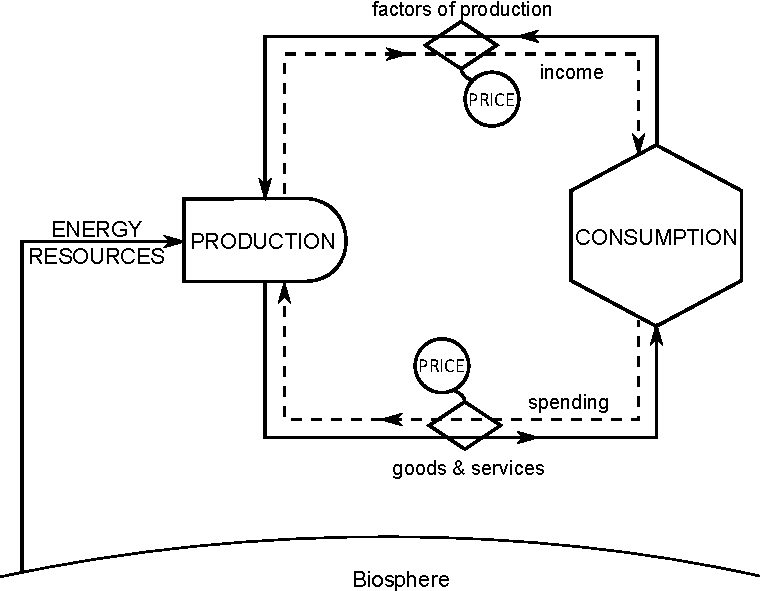
\includegraphics[width=\linewidth]{Part_0/Chapter_Introduction/images/Perpetual_motion_2.pdf}
\caption[The traditional model supplemented with resource inputs]{Energy and material input output analysis has included the flows into the economy from the environment. This may be considered a perpetual motion machine of the second kind.[SHOULD FLOW FROM `RAW RESOURCES' ALSO GO STRAIGHT INTO CONSUMPTION?}
\end{figure}

\begin{figure}[!ht]
\centering{}
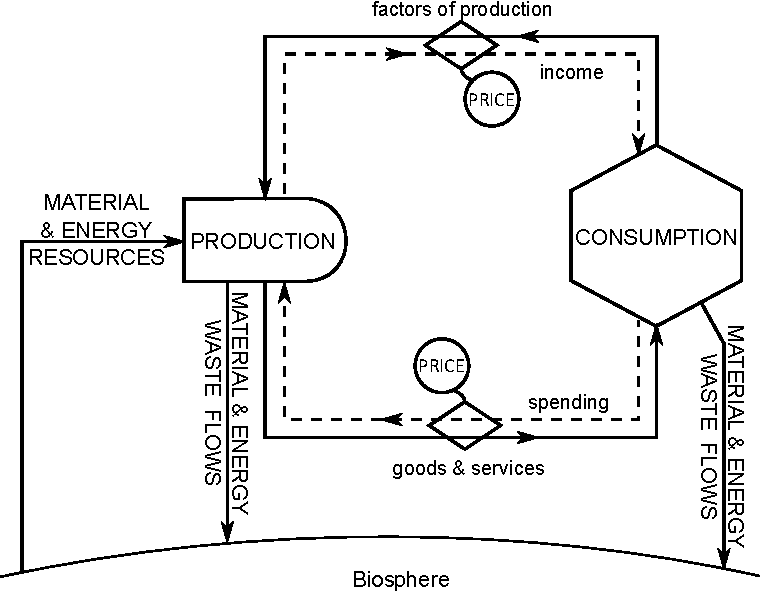
\includegraphics[width=\linewidth]{Part_0/Chapter_Introduction/images/PERKS.pdf}
\caption[A comprehensive biophysical (?) model of the economy]{A comprehensive model of the economy, fully consistent with the laws of thermodynamics must include degraded resources (waste) expelled to the environment as a necessary consequence of economic activity.}
\end{figure}

\begin{figure}[!ht]
\centering{}
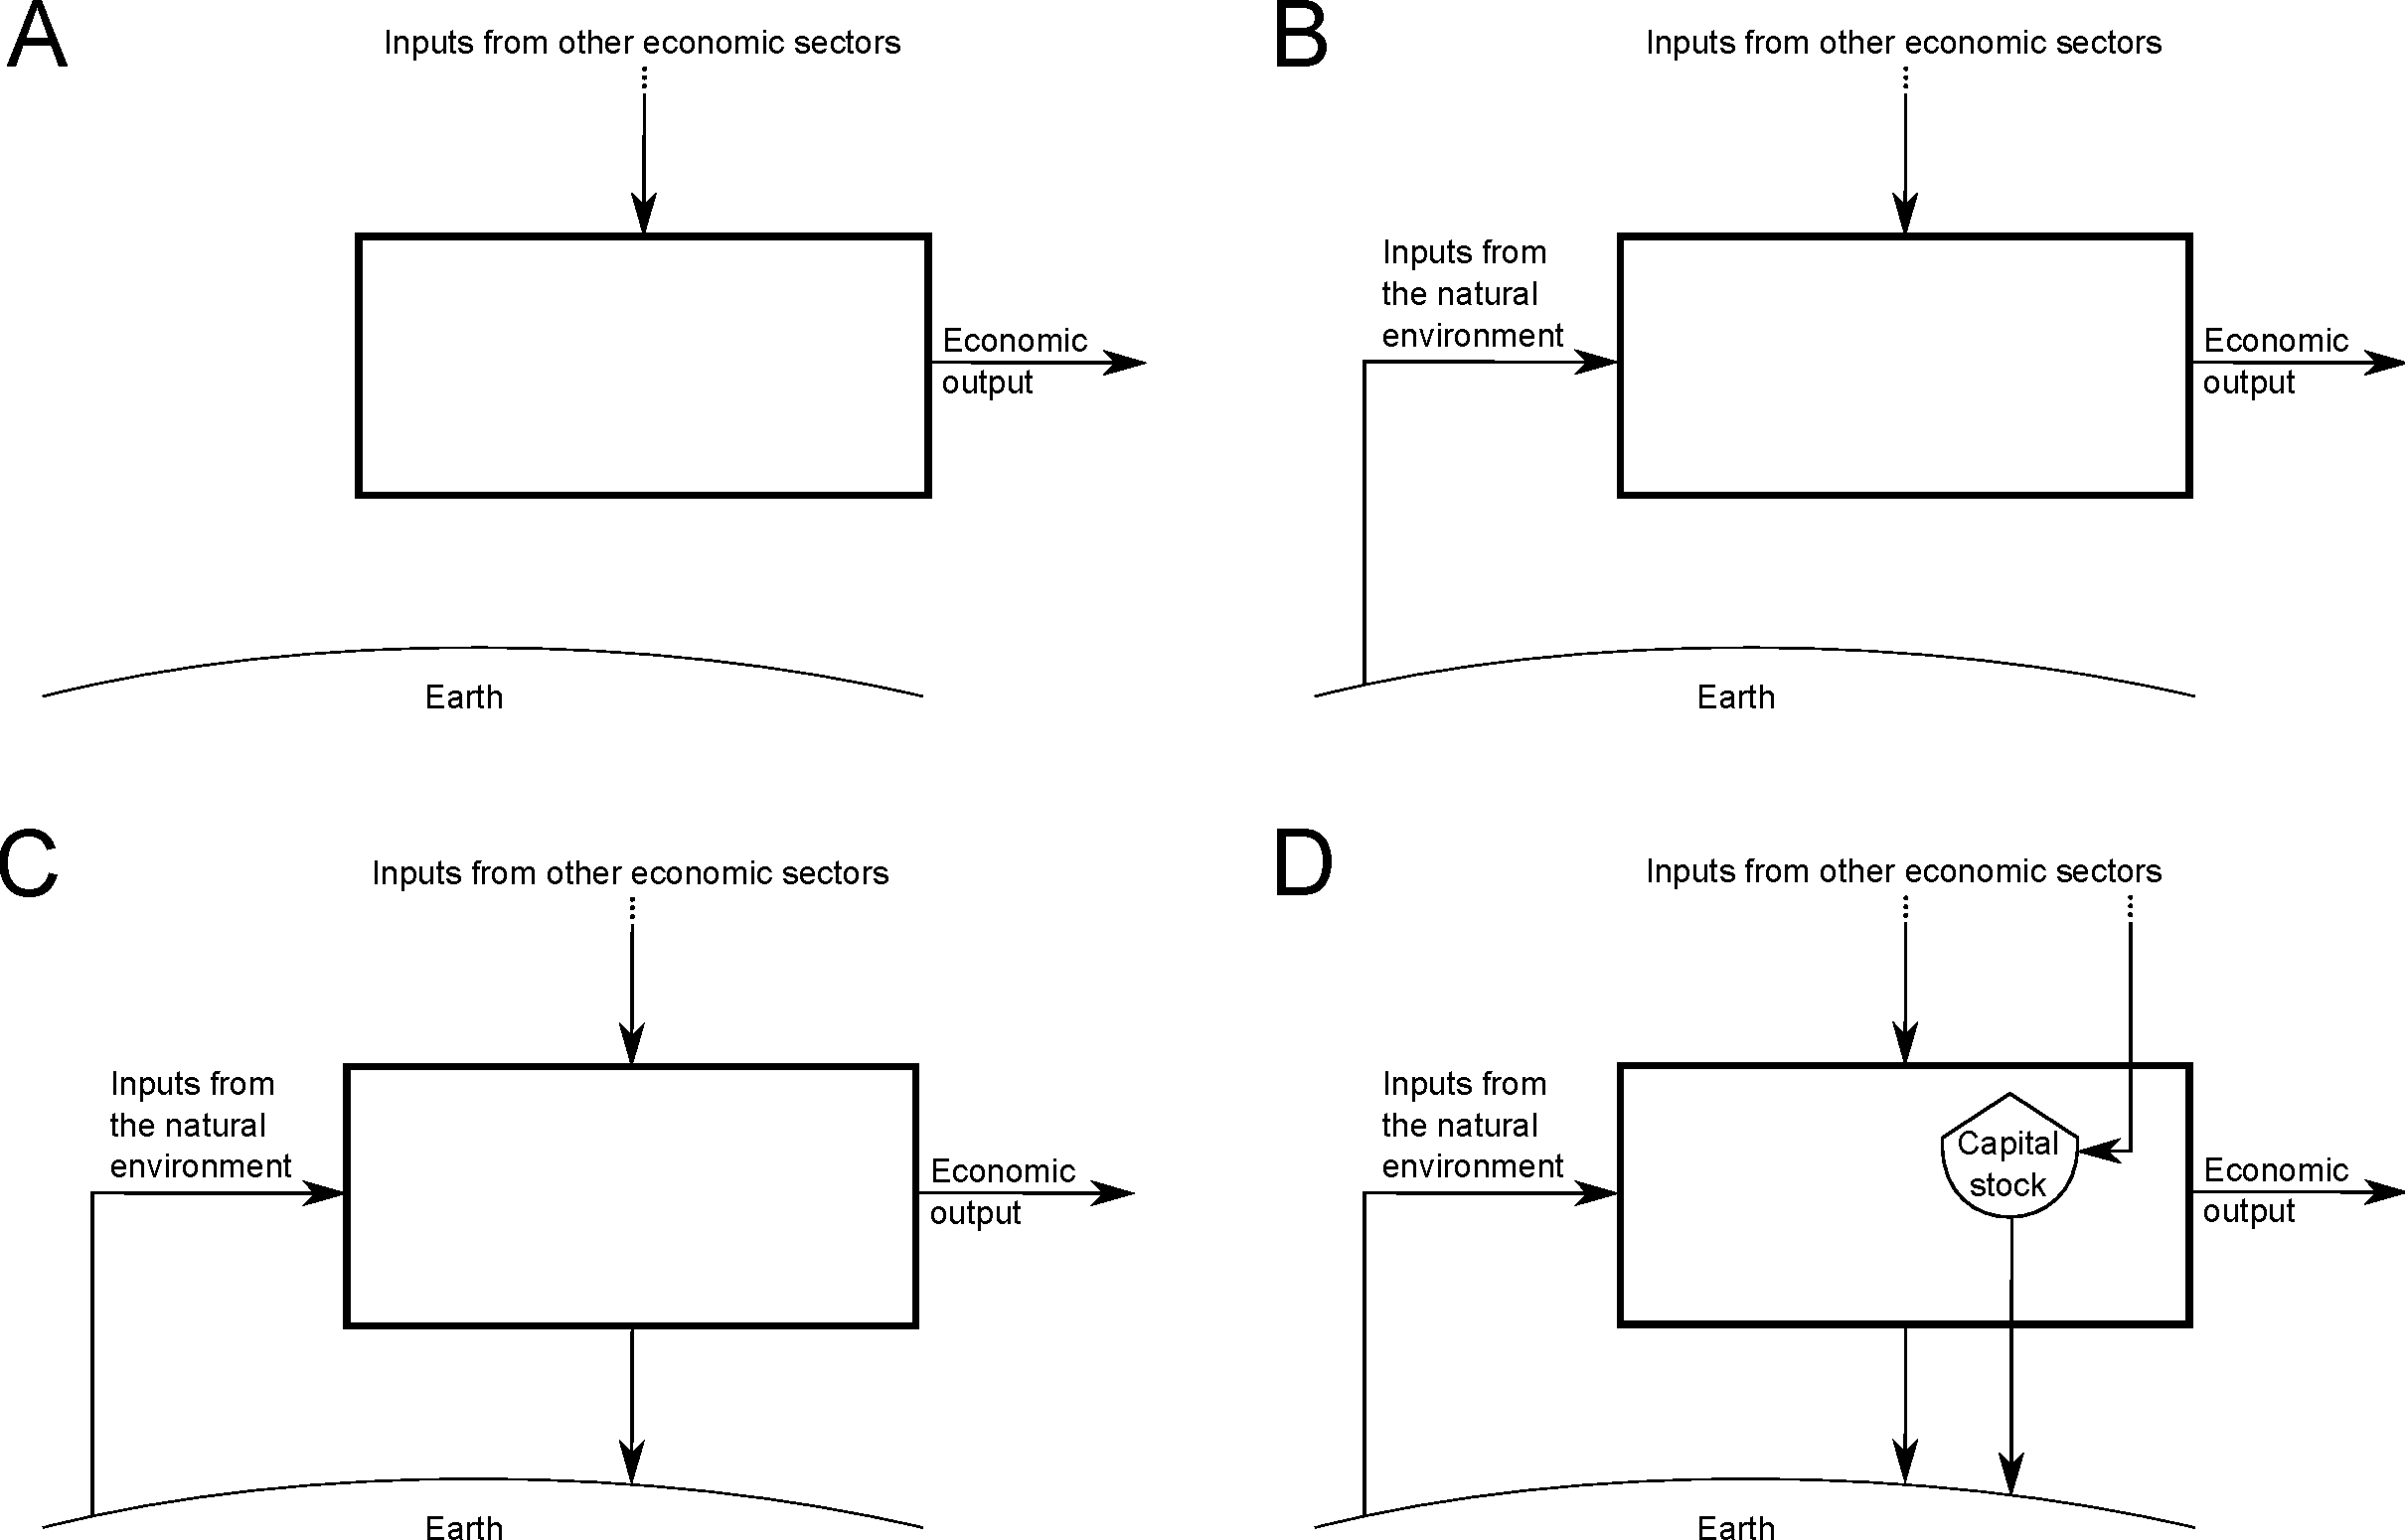
\includegraphics[width=\linewidth]{Part_0/Chapter_Introduction/images/Basic_unit_square.pdf}
\caption[The basic unit of input-output modeling]{The basic unit of input-output modeling: \textbf{A} the standard economic approach includes only transactions among sectors of the economy; \textbf{B} the ecological economics approach models inputs from the natural environment outside the economy as factors of production; \textbf{C} including waste flows to the environment makes the model physically consistent and; \textbf{D} the method presented here accounts also for accumulation, K, of embodied energy within materials in economic sectors. [SHOULD WE HAVE THE LABEL ``K'' IN THE ACCUMULATION, OR JUST HAVE THE TANK?]}
\label{fig:basic_unit}
\end{figure}
%\section{Issues of resource quality}
%
%[DO WE NEED THIS SECTION? IT FEELS LIKE WE SHOULD MOVE FROM THE PREVIOUS SECTION WHEREIN WE CLEARLY DEMONSTRATE THE NEED FOR OUR WORK TO BEGINNING THE PROCESS OF DEVELOPING THE METHOD. IF WE WANT TO KEEP THIS SECTION, WE SHOULD DO A BETTER JOB AT SHOWING WHY IT IS NEEDED. WE SHOULD POINT BACK TO BULLARD AND HERENDEEN AND SAY THAT THEIR METHOD DOESN'T ACCOUNT FOR DECREASING RESOURCE QUALITY AND WHY A METHOD IS NEEDED THAT DOES ACCOUNT FOR DECLINING RESOURCE QUALITY. --MKH] Raw material and energy resources must first be extracted from the natural environment before they may be utilized in the economy to provide goods and service to society. Despite increasing levels of technological efficiency, for example in consumer goods such as refrigerators and cars, evidence shows that the energy intensity of primary resource extraction, i.e. the energy required to extract raw materials from the environment, has been steadily increasing over the last fifty years \cite{Hall1986, Mudd2010, Brandt2011}. This increasing energy requirement for primary extraction means that less \textit{net energy} is available for downstream uses. If this decline in net energy availability outpaces technological advances in energy efficiency, there may be deleterious impacts on the economic output of the economy.

\section{An I-O method for dynamic (transient) economic analysis}

In this paper, we develop a physical input-output, matrix-based method for modeling multi-sector economies, in the tradition of Georgescu-Roegen's ``flow-fund'' model \cite{G-R1979a, G-R1979b}. The method presented in this paper takes a decidedly engineering approach **** Need to re-cast in metabolic language !!!! **** to extend the techniques of Bullard, Herendeen, and others to account for durability of goods and embodied energy. This method allows us to see how energy and materials flow through the economy, where embodied energy accumulates in the economy, and how declining resource quality may affect these dynamics. [NEED TO MAKE SURE WE ACHIEVE THIS LAST POINT]

This paper is organized as follows. We first discuss methodology and the model economy. Thereafter, we present three examples, each with increasing levels of disaggregation among society, the energy sector, and goods and services sectors, culminating with a matrix formulation of the new method. The examples leverage the First Law of Thermodynamics, account for total energy (($T$), and develop accounting relationships for embodied energy ($B$). Within the examples, we develop a precise definition for embodied energy and a matrix formulation of the method that can be extended to an arbitrarily large number of economic sectors. Finally, we draw several implications from the development of the new method.


\bibliographystyle{unsrt}
\bibliography{../../EROI_review_v2}


% Always give a unique label
% and use \ref{<label>} for cross-references
% and \cite{<label>} for bibliographic references
% use \sectionmark{}
% to alter or adjust the section heading in the running head
%% Instead of simply listing headings of different levels we recommend to let every heading be followed by at least a short passage of text. Furtheron please use the \LaTeX\ automatism for all your cross-references and citations.

%% Please note that the first line of text that follows a heading is not indented, whereas the first lines of all sequent paragraphs are.

%% Use the standard \verb|equation| environment to typeset your equations, e.g.
%
%% \begin{equation}
%% a \times b = c\;,
%% \end{equation}
%
%% however, for multiline equations we recommend to use the \verb|eqnarray|
%% environment\footnote{In physics texts please activate the class option \texttt{vecphys} to depict your vectors in \textbf{\itshape boldface-italic} type - as is customary for a wide range of physical jects.}.
%% \begin{eqnarray}
%% a \times b = c \nonumber\\
%% \vec{a} \cdot \vec{b}=\vec{c}
%% \label{eq:01}
%% \end{eqnarray}

%% \section{section Heading}
%% \label{sec:2}
%% Instead of simply listing headings of different levels we recommend to let every heading be followed by at least a short passage of text. Furtheron please use the \LaTeX\ automatism for all your cross-references\index{cross-references} and citations\index{citations} as has already been described in Sect.~\ref{sec:2}.

%% \begin{quotation}
%% Please do not use quotation marks when quoting texts! Simply use the \verb|quotation| environment -- it will automatically render Springer's preferred layout.
%% \end{quotation}


%% \section{section Heading}
%% Instead of simply listing headings of different levels we recommend to let every heading be followed by at least a short passage of text. Furtheron please use the \LaTeX\ automatism for all your cross-references and citations as has already been described in Sect.~\ref{sec:2}, see also Fig.~\ref{fig:1}\footnote{If you copy text passages, figures, or tables from other works, you must obtain \textit{permission} from the copyright holder (usually the original publisher). Please enclose the signed permission with the manucript. The sources\index{permission to print} must be acknowledged either in the captions, as footnotes or in a separate section of the book.}

%% Please note that the first line of text that follows a heading is not indented, whereas the first lines of all sequent paragraphs are.

% For figures use
%
%% \begin{figure}[b]
%% \sidecaption
% Use the relevant command for your figure-insertion program
% to insert the figure file.
% For example, with the option graphics use
%% \includegraphics[scale=.65]{figure}
%
% If not, use
%\picplace{5cm}{2cm} % Give the correct figure height and width in cm
%
%% \caption{If the width of the figure is less than 7.8 cm use the \texttt{sidecapion} command to flush the caption on the left side of the page. If the figure is positioned at the top of the page, align the sidecaption with the top of the figure -- to achieve this you simply need to use the optional argument \texttt{[t]} with the \texttt{sidecaption} command}
%% \label{fig:1}       % Give a unique label
%% \end{figure}


%% \paragraph{Paragraph Heading} %
%% Instead of simply listing headings of different levels we recommend to let every heading be followed by at least a short passage of text. Furtheron please use the \LaTeX\ automatism for all your cross-references and citations as has already been described in Sect.~\ref{sec:2}.

%% Please note that the first line of text that follows a heading is not indented, whereas the first lines of all sequent paragraphs are.

%% For typesetting numbered lists we recommend to use the \verb|enumerate| environment -- it will automatically render Springer's preferred layout.

%% \begin{enumerate}
%% \item{Livelihood and survival mobility are oftentimes coutcomes of uneven socioeconomic development.}
%% \begin{enumerate}
%% \item{Livelihood and survival mobility are oftentimes coutcomes of uneven socioeconomic development.}
%% \item{Livelihood and survival mobility are oftentimes coutcomes of uneven socioeconomic development.}
%% \end{enumerate}
%% \item{Livelihood and survival mobility are oftentimes coutcomes of uneven socioeconomic development.}
%% \end{enumerate}


%% \paragraph{paragraph Heading} In order to avoid simply listing headings of different levels we recommend to let every heading be followed by at least a short passage of text. Use the \LaTeX\ automatism for all your cross-references and citations as has already been described in Sect.~\ref{sec:2}, see also Fig.~\ref{fig:2}.

%% Please note that the first line of text that follows a heading is not indented, whereas the first lines of all sequent paragraphs are.

%% For unnumbered list we recommend to use the \verb|itemize| environment -- it will automatically render Springer's preferred layout.

%% \begin{itemize}
%% \item{Livelihood and survival mobility are oftentimes coutcomes of uneven socioeconomic development, cf. Table~\ref{tab:1}.}
%% \begin{itemize}
%% \item{Livelihood and survival mobility are oftentimes coutcomes of uneven socioeconomic development.}
%% \item{Livelihood and survival mobility are oftentimes coutcomes of uneven socioeconomic development.}
%% \end{itemize}
%% \item{Livelihood and survival mobility are oftentimes coutcomes of uneven socioeconomic development.}
%% \end{itemize}

%% \begin{figure}[t]
%% \sidecaption[t]
% Use the relevant command for your figure-insertion program
% to insert the figure file.
% For example, with the option graphics use
%% \includegraphics[scale=.65]{figure}
%
% If not, use
%\picplace{5cm}{2cm} % Give the correct figure height and width in cm
%
%% \caption{Please write your figure caption here}
%% \label{fig:2}       % Give a unique label
%% \end{figure}

%% \runinhead{Run-in Heading Boldface Version} Use the \LaTeX\ automatism for all your cross-references and citations as has already been described in Sect.~\ref{sec:2}.

%% \runinhead{Run-in Heading Italic Version} Use the \LaTeX\ automatism for all your cross-refer\-ences and citations as has already been described in Sect.~\ref{sec:2}\index{paragraph}.
% Use the \index{} command to code your index words
%
% For tables use
%
%% \begin{table}
%% \caption{Please write your table caption here}
%% \label{tab:1}       % Give a unique label
%
% For LaTeX tables use
%
%% \begin{tabular}{p{2cm}p{2.4cm}p{2cm}p{4.9cm}}
%% \hline\noalign{\smallskip}
%% Classes & class & Length & Action Mechanism  \\
%% \noalign{\smallskip}\svhline\noalign{\smallskip}
%% Translation & mRNA$^a$  & 22 (19--25) & Translation repression, mRNA cleavage\\
%% Translation & mRNA cleavage & 21 & mRNA cleavage\\
%% Translation & mRNA  & 21--22 & mRNA cleavage\\
%%Translation & mRNA  & 24--26 & Histone and DNA Modification\\
%%\noalign{\smallskip}\hline\noalign{\smallskip}
%%\end{tabular}
%%$^a$ Table foot note (with superscript)
%%\end{table}
%
%% \section{Section Heading}
%%\label{sec:3}
% Always give a unique label
% and use \ref{<label>} for cross-references
% and \cite{<label>} for bibliographic references
% use \sectionmark{}
% to alter or adjust the section heading in the running head
%% Instead of simply listing headings of different levels we recommend to let every heading be followed by at least a short passage of text. Furtheron please use the \LaTeX\ automatism for all your cross-references and citations as has already been described in Sect.~\ref{sec:2}.

%% Please note that the first line of text that follows a heading is not indented, whereas the first lines of all sequent paragraphs are.

%%If you want to list definitions or the like we recommend to use the Springer-enhanced \verb|description| environment -- it will automatically render Springer's preferred layout.

%%\begin{description}[Type 1]
%%\item[Type 1]{That addresses central themes pertainng to migration, health, and disease. In Sect.~\ref{sec:1}, Wilson discusses the role of human migration in infectious disease distributions and patterns.}
%%\item[Type 2]{That addresses central themes pertainng to migration, health, and disease. In Sect.~\ref{sec:2}, Wilson discusses the role of human migration in infectious disease distributions and patterns.}
%%\end{description}

%%\section{section Heading} %
%% In order to avoid simply listing headings of different levels we recommend to let every heading be followed by at least a short passage of text. Use the \LaTeX\ automatism for all your cross-references and citations citations as has already been described in Sect.~\ref{sec:2}.

%% Please note that the first line of text that follows a heading is not indented, whereas the first lines of all sequent paragraphs are.

%% \begin{svgraybox}
%% If you want to emphasize complete paragraphs of texts we recommend to use the newly defined Springer class option \verb|graybox| and the newly defined environment \verb|svgraybox|. This will produce a 15 percent screened box 'behind' your text.

%% If you want to emphasize complete paragraphs of texts we recommend to use the newly defined Springer class option and environment \verb|svgraybox|. This will produce a 15 percent screened box 'behind' your text.
%% \end{svgraybox}


%% \section{section Heading}
%%Instead of simply listing headings of different levels we recommend to let every heading be followed by at least a short passage of text. Furtheron please use the \LaTeX\ automatism for all your cross-references and citations as has already been described in Sect.~\ref{sec:2}.

%% Please note that the first line of text that follows a heading is not indented, whereas the first lines of all sequent paragraphs are.

%% \begin{theorem}
%% Theorem text goes here.
%% \end{theorem}
%
% or
%
%% \begin{definition}
%% Definition text goes here.
%% \end{definition}

%% \begin{proof}
%\smartqed
%% Proof text goes here.
%% \qed
%% \end{proof}

%%\paragraph{Paragraph Heading} %
%% Instead of simply listing headings of different levels we recommend to let every heading be followed by at least a short passage of text. Furtheron please use the \LaTeX\ automatism for all your cross-references and citations as has already been described in Sect.~\ref{sec:2}.

%% Note that the first line of text that follows a heading is not indented, whereas the first lines of all subsequent paragraphs are.
%
% For built-in environments use
%
%%\begin{theorem}
%%Theorem text goes here.
%%\end{theorem}
%
%%\begin{definition}
%%Definition text goes here.
%%\end{definition}
%
%%\begin{proof}
%%\smartqed
%% Proof text goes here.
%%\qed
%%\end{proof}
%
%% \begin{acknowledgement}
%% If you want to include acknowledgments of assistance and the like at the end of an individual chapter please use the \verb|acknowledgement| environment -- it will automatically render Springer's preferred layout.
%% \end{acknowledgement}
%
%% \section*{Appendix}
%% \addcontentsline{toc}{section}{Appendix}
%
%% When placed at the end of a chapter or contribution (as opposed to at the end of the book), the numbering of tables, figures, and equations in the appendix section continues on from that in the main text. Hence please \textit{do not} use the \verb|appendix| command when writing an appendix at the end of your chapter or contribution. If there is only one the appendix is designated ``Appendix'', or ``Appendix 1'', or ``Appendix 2'', etc. if there is more than one.

%% \begin{equation}
%% a \times b = c
%% \end{equation}
% Problems or Exercises should be sorted chapterwise
%% \section*{Problems}
%% \addcontentsline{toc}{section}{Problems}
%
% Use the following environment.
% Don't forget to label each problem;
% the label is needed for the solutions' environment
%% \begin{prob}
%% \label{prob1}
%% A given problem or Excercise is described here. The
%% problem is described here. The problem is described here.
%% \end{prob}

%% \begin{prob}
%% \label{prob2}
%% \textbf{Problem Heading}\\
%% (a) The first part of the problem is described here.\\
%% (b) The second part of the problem is described here.
%% \end{prob}


